%!TEX root =/Users/ludovicl/Dropbox/Cours/UTBM/P15/RapportStage/main.tex
\chapter{Mise en situation et description des activités du stagiaire}


\section{Création d'une front pour l'importation des données de billetteries clients}

L'une de mes premières taches en arrivant dans l'entreprise est de créer un front-end permettant à Tech4Team et à certains clients de facilement insérer en base de données un fichier CSV\footnote{Comma-separated values, connu sous le sigle CSV, est un format informatique ouvert représentant des données tabulaires sous forme de valeurs séparées par des virgules.} contenant des données billetteries.

\subsection{Le besoin}

Le besoin peut donc être visualisé par le schéma \ref{interface_upload} page \pageref{interface_upload}. Tech4Team ou un client veut insérer des nouveaux tickets dans la base de données Arenapricing. Il sélectionne alors un fichier CSV à la main depuis l'interface web, spécifie le type de logiciel billetterie ayant permis de générer le fichier et clique sur envoyer. Le site analyse le fichier, extrait les informations importantes et les inserts en base de donnes. Toute la partie d'analyse et d'insertion doit être invisible du point de vue de l'utilisateur. 

\begin{center}

\includegraphics[scale=0.6]{images/datafit.png}
\captionof{figure}{Principe de l'interface d'upload}
\label{interface_upload}
\end{center}


\subsection{Le front d'importation de manières technique}

Pour réaliser ce site web d'importation nous avons décidé après discussion avec le lead developper d'utiliser le langage Python. Ce langage permet de développer rapidement est dispose d'énormément de modules s'ajoutant aux fonctions de base. Il est ainsi aisé de parser un fichier CSV. J'ai également utilisé le microframework Flask pour créer les pages web en elle même et servir de serveur web. Pour le design du site, j'ai utilisé le framework Zurb Foundation afin d'avoir une identité visuelle cohérente. 

\begin{center}
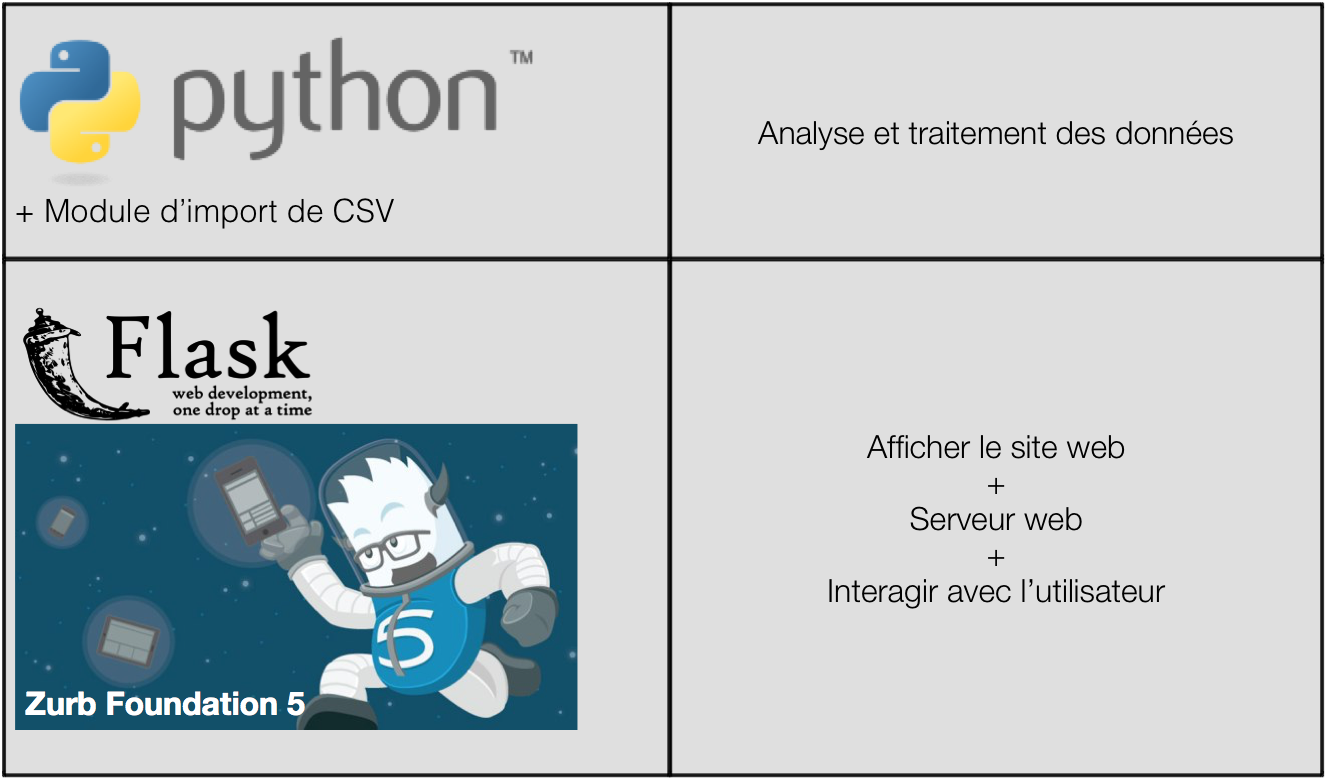
\includegraphics[scale=0.7]{images/datafit2.png}
\captionof{figure}{Téchnologies utilisées pour le front}
\label{interface_upload_tech}
\end{center}

\subsection{Résultats obtenus}

Comme nous pouvons le voir sur l'impression d'écran \ref{front_upload} page \pageref{front_upload} l'interface est simple et permet à l'utilisateur de faire l'essentiel, c'est-à-dire envoyer sont fichier csv préalablement sélectionné.
En plus du nom de l'organisation, nous affichons le type d'événement correspondant au fichier envoyé ainsi que le logiciel de billetterie d'où provient l'export. \\

\subsubsection{Upload d'un fichier}

L'impression d'écran \ref{front_orga} page \pageref{front_orga} permet de visualiser l'interface de création d'une nouvelle organisation. Il est en effet possible pour l'utilisateur de créer une nouvelle organisation en choisissant les données suivantes.

\begin{center}
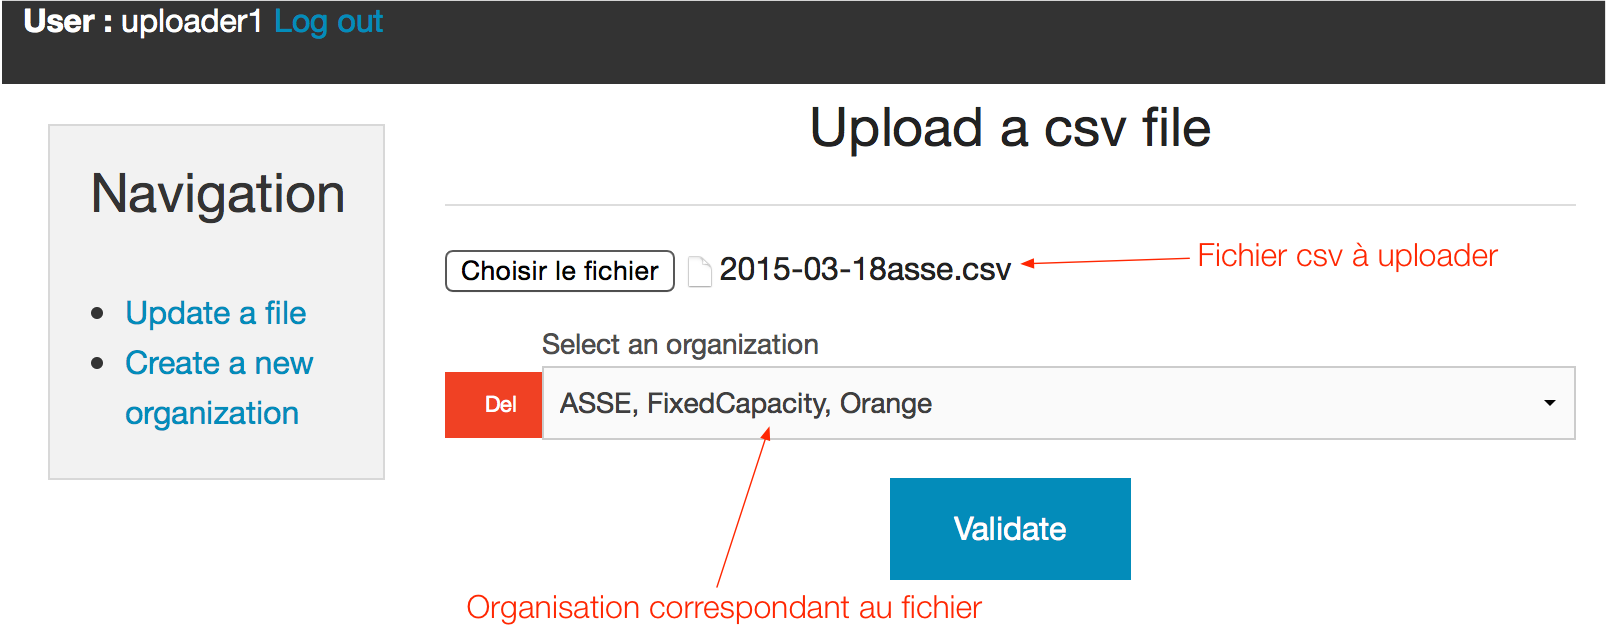
\includegraphics[scale=0.6]{images/front1.png}
\captionof{figure}{Front d'upload d'un fichier CSV}
\label{front_upload}
\end{center}


\subsubsection{Création d'une organisation}

Comme le montre l'impression d'écran \ref{front_orga} page \pageref{front_orga} la seconde page de ce site d'upload permet à l'utilisateur de créer une nouvelle organisation. 

Une organisation est caractérisée par plusieurs choses : 

\begin{itemize}
	\item[\textbullet] Le type d'événement organisé par l'organisation :
	\begin{itemize}
  		\item FixedCapacity : c'est à dire que la placement est fixe est indiqué sur le ticket, c'est le cas pour les matchs de foot où les pièces théâtres.
		\item FreeCapacity : c'est-à-dire que le placement est libre, l'utilisateur n'a pas de place définie sur son ticket, c'est les marathons et les salons.
	\end{itemize}
	\item[\textbullet] Le nom du logiciel de billetterie qu'utilise l'organisation (DataSport, Weezevent, Orange,...)
	\item[\textbullet] Le nom de l'organisation, qui sera ensuite affiché sur le site de visualisation des ventes de tickets.
\end{itemize}

\begin{center}
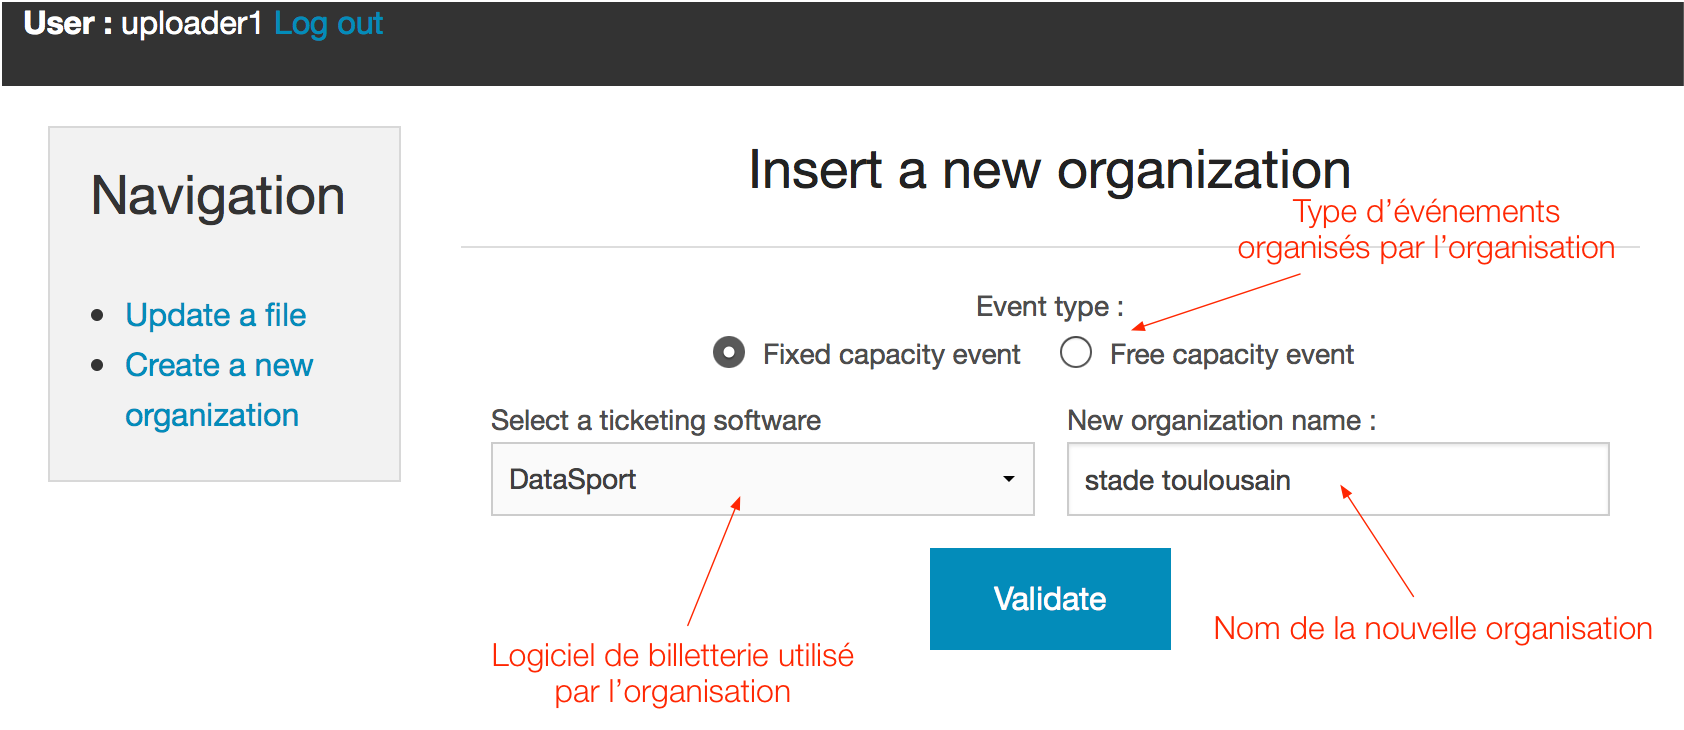
\includegraphics[scale=0.55]{images/front2.png}
\captionof{figure}{Front de création d'une organisation}
\label{front_orga}
\end{center}

Toutes les données rentrées par l'utilisateur ainsi que les comptes utilisateurs sont inscrites dans une base de données PostgreSQL. Pour faire les insertions et les sélections en base de données, j'utilise l'ORM SQLAlchemy.

\section{Back-end de l'importation des données de billéteries}
\subsection{Les fichiers CSV}
La majorité des des clients nous fournissent des fichiers CSV. Ces fichiers sont extraits à partir du logiciel de billéterie utilisé par le client.

Comme le montre l'image \ref{eg_csv} page \pageref{eg_csv} les données nous permette de récuperer le nom de l'évenement (ici Les Parapluies de Cherbourg), la date de l'événement, le prix ainsi que la date d'achat du ticket,...

En fonction des données de billéteries que nous récupérons nous pouvons églement récupérer le mail, nom, prénom, adresse des utilisateur. Cela nous permet d'agrémenter notre logiciel de CRM. %TODO : Parler de arenapublic

\begin{center}
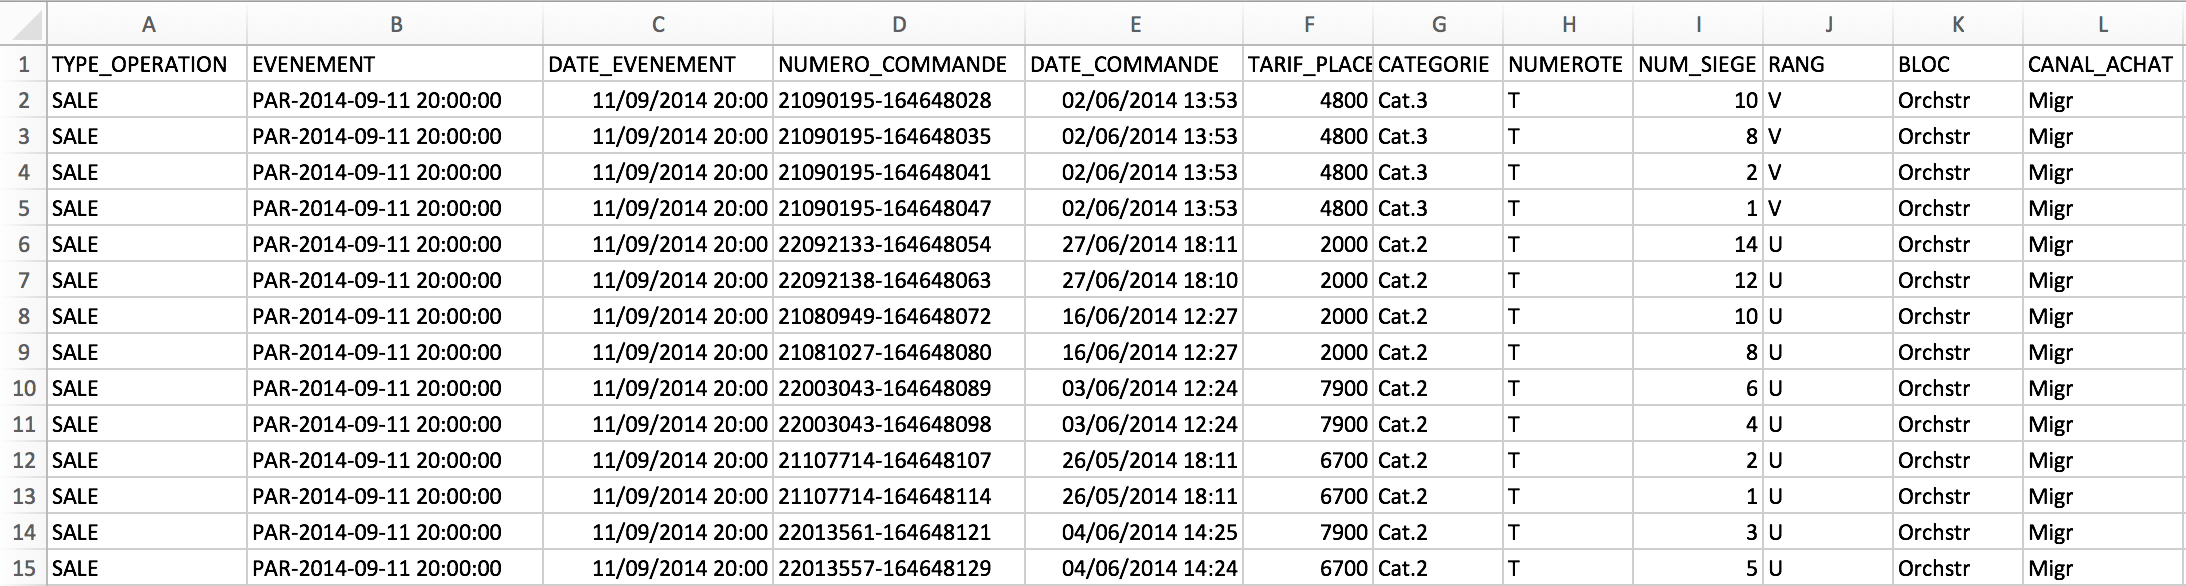
\includegraphics[scale=0.45]{Images/eg_csv1}
\captionof{figure}{Example de fichier CSV fournis par le théâtre du Chatelet}
\label{eg_csv}
\end{center}

\subsubsection{Parsing des données en Python}
Pour parser les fichiers CSV j'ai utilise le module natif CSV. 


\lstset{style=custompython}
\begin{lstlisting}
with open(p_path_file, 'r', encoding=charset['encoding']) as f:

	#read csv file with csv module
	dict_csv = csv.DictReader(f, delimiter=';', quoting=csv.QUOTE_ALL)
	
	#use strategy design pattern with Secutix object
	secutix = ParsingStrategyContext(Secutix())	
	
	#parse dictionay with organization name, event date, export date
	secutix.parse_file(dict_csv, o_name, e_date, export_date)

#ask object to send data to the ruby. e_type is event type 
reason = secutix.upload_data(e_type)
return reason
\end{lstlisting}


















